%----------------------------------------------------------------------------------------
%	PACKAGES AND OTHER DOCUMENT CONFIGURATIONS
%----------------------------------------------------------------------------------------

\documentclass[12pt]{article} 
\usepackage{geometry} 
\geometry{a4paper, textheight=705pt} 
\usepackage{graphicx}
\usepackage{float} 
\linespread{1.2} 
\DeclareGraphicsExtensions{.png}
\usepackage[none]{hyphenat}
\usepackage{pdflscape}

%----------------------------------------------------------------------------------------
%	TITLE PAGE
%----------------------------------------------------------------------------------------

\begin{document}

\begin{titlepage}

\newcommand{\HRule}{\rule{\linewidth}{0.5mm}} 

\center


\includegraphics{aber}\\[1cm] 

\textsc{\Large Computer Science}\\[0.5cm] 

\HRule \\[0.8cm]
{ \huge \bfseries Industrial Year Report}\\[0.4cm]
\HRule \\[1.5cm]

\begin{minipage}{0.4\textwidth}
\begin{flushleft} \large
\emph{Author:}\\
Craig \textsc{Heptinstall}
\end{flushleft}
\end{minipage}
~
\begin{minipage}{0.4\textwidth}
\begin{flushright} \large
\emph{Supervisor:} \\
Dr. Richard \textsc{Shipman}
\end{flushright}
\end{minipage}\\[0.2cm]
%-------------------------------
\begin{minipage}{0.85\textwidth}
\begin{flushleft} \large
\emph{Aber-User:}\\
(Crh13)
\end{flushleft}
\end{minipage}\\[8cm]
%-------------------------------
\begin{minipage}{0.28\textwidth}
{\large \today}\\
\large \emph{V2.0 Final}
\end{minipage}\\[2cm]
%-------------------------------

\vfill

\end{titlepage}

\pagestyle{myheadings}
\markright{Craig Heptinstall (Crh13)\hfill Industrial Year Report\hfill}
%----------------------------------------------------------------------------------------
%	TABLE OF CONTENTS
%----------------------------------------------------------------------------------------
\setcounter{page}{2}
\tableofcontents

\newpage

%----------------------------------------------------------------------------------------
%	INTRODUCTION
%----------------------------------------------------------------------------------------

\section{Introduction}
This report is intended to provide a detailed context and evaluation of the industrial year placement opportunity I
completed over the past year, and to give the reader of this document an idea of my experiences at and away from my
workplace. A description of my placement is presented first, and is then expanded by a look at the organisational
environment of the company and department I was based at. This is then followed by a more detailed look at the actual
work carried out, from the technical aspects to the application environments used at the work place. Furthermore, I have
then also outlined the work I carried out personally and as a team whilst working on my placement, and the social
aspects of where I worked. In terms of a summary of this report, there is a critical evaluation section providing detail
towards how I felt I improved at my skills, and where I thought the placement was good or not so good.\\ \par \noindent
Before I begin this report, I would first like to mention and comment upon how I handled seeking and applying for jobs,
leading to the placement I had. I first began searching for placements at the begging of summer the year before the
start of a placement, as to give myself a good amount of time to find and apply to as many good placements as possible.
Over the academic year I had sent numerous applications out, aiming towards the software development/ web development
area. As a Software Engineering MEng student, I knew that primarily software based jobs would be more ideal.\\ \par \noindent
I found the competition for most jobs to be quiet intense, where in some cases along with myself, employers would be
interviewing between from five to over thirty other applicants. After several unsuccessful attempts coming from
interviews, I did find myself a little disheartened as the date to find a placement grew closer. I learnt a great deal
during all this process, especially towards self-confidence and interview skills. The placement I got accepted from came
through a university advertisement, where a previous student the year before had worked, and having the employer being
impressed so much they had asked for another.\\ \par\noindent
When I initially saw the job advertisement, because this placement was abroad, and concentrated on both programming and
some web development, this instantly attracted me and I decided to apply for it. As with other placements I applied for,
I had an interview, but this time on-line due to the distance of the company. I was surprised during this interview the
lesser amount of technical questions, but instead personality and more social questions. I was offered the job at
the start of April, though still gave me eight weeks to prepare and move to another country, while still
preparing for exams. Job specifics are in the next section of this report.
%------------------------------------------------

%----------------------------------------------------------------------------------------
%	Organisational Environment Description 
%----------------------------------------------------------------------------------------

\section{Organisational Environment Description}
This section goes into detail about the job specifics, location and the employer I worked for whilst at my industrial
placement. The job I was offered was as a Software Developer of a JavaEE application at a German company named Plunet,
the software relating to business and project management. This was primarily a web application named BusinessManager
that would allow creation, workflow management and the handling of processes from requests through to invoicing of
translation and localisation projects. For instance, some companies have departments devoted to translations of
important documents, manuals and anything else that needs translation, and in order to do this they usually use
translators and CAT (Computer aided translation) tools. The purpose of the software I worked on (BusinessManager) was to
provide an efficient means of allowing translation teams to incorporate the whole process of this type of transition,
and also to allow the linking between these CAT tools and the software so users could directly translate documents.\\ \par \noindent
In addition to this, the application was also used as a means of translation companies connecting to their clients,
where the clients would create ‘requests’ inside the application, and then this would be directly accepted by the
translation company through BusinessManager and turned into a ‘quote’. The process of retrieving files, uploading them
to any of the various CAT tools (included MemoQ, SDL Trados, XTM, MemSource, DVX and Transit)  
the company would have active, and then when translation was complete, an invoice could
be crated and given to the customer along with the completed files. This all integrated into the web interface of the
software, which I worked on along with various back-end tasks. The BusinessManager software is used by localization
teams and translation companies around the world, having some large clients including Siemens.\\ \par \noindent
Looking into more at my role at the company, I was assigned to the CAT team, a team of 3-4 developers devoted to the
linkage between BusinessManager and CAT tools. In my role I was assigned bug fixes, along with implementations of new
features and even new integrations with more CAT tools (There is more detail to this in the description of work I
carried out, section 4). My department was headed by one developer, who I reported to directly throughout my year in
industry, and who was responsible for overseeing my work, and providing any evaluations of my work when necessary.
Concentrating more on the company itself, Plunet is a company based in the Berlin, Germany. The BusinessManager software
provided by the company was originally created by a company; EDVK Konzpte, but was eventually branched off and created
into a new company when it grew. Because Plunet has been growing more and more in recent years, the company actually has
two main places of work, one of which in Würzburg, southern Germany is where the development is based and also where I
was based throughout this year. While the Würzburg office is for development, the Berlin office is aimed towards sales
and more corporate means.\\ \par \noindent
Starting with the Berlin office, this is led by the CEO and part owner of the organisation who oversees the business
strategy and overall company management. There is also the sales and marketing team in Berlin, with the sales team
responsible for meetings with current and potential clients through webinars (online video displays of the application).
Sales team members are also closely linked with the development team in Würzburg, to give feedback directly about new
implementations, or any changes they would suggest whether it being new features or existing bugs found in the software.
The marketing team are more towards the web presence and social networking of the application e.g. the Plunet website,
Twitter etc.\\ \par \noindent
Looking at the second office (Figure~\ref{fig:test}), where I was incorporated the development team is firstly split into three departments: the
developer and customer support team, the CAT team, and other developers working on the rest of the BusinessManager
application (though this has various subsets of departments, such as the GUI(interface of the web application), and
specific parts of the application such as emailing functionality, though these small departments can change depending on
task priority at the time).

\begin{figure}[ht]
    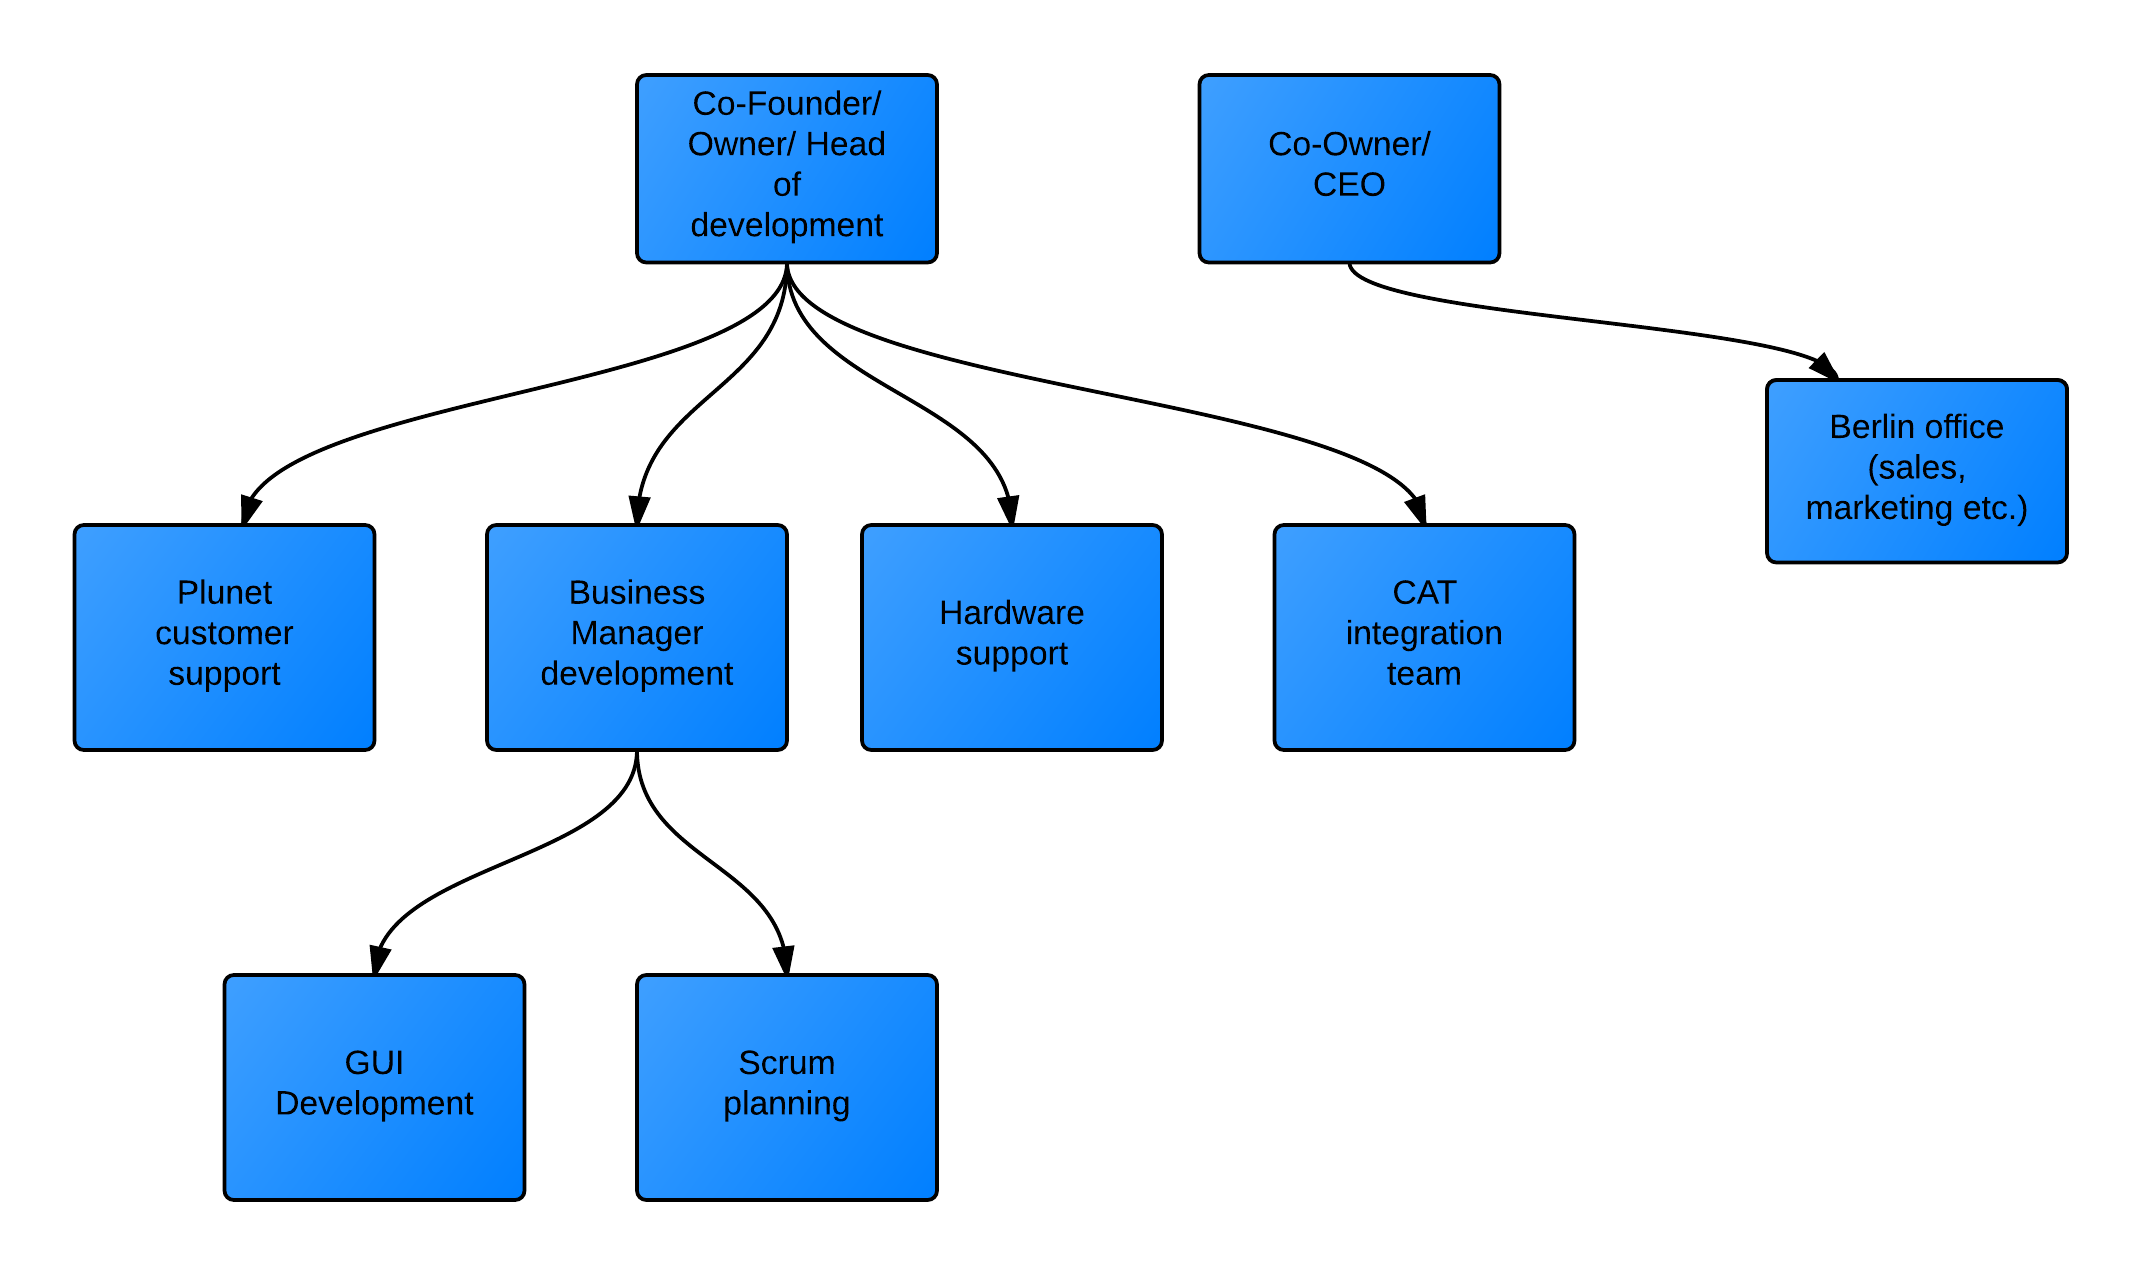
\includegraphics[scale=0.2]{ranks}
    \caption{Structure of staff at Wurzburg office.}
     \label{fig:test}
\end{figure}

%------------------------------------------------

%----------------------------------------------------------------------------------------
%    Technical And Applications Environments Description
%----------------------------------------------------------------------------------------

\section{Description of The Technical and Applications Environment}
This section looks at the development environments, languages and other key software I used during my industrial year.
Starting with the actual equipment and operating systems used, the office used windows for both development systems and
also server machines used to host the application and also to host some of the CAT tools. When I had just arrived at the
office, some of the development machines had recently been upgraded to deal with the higher requirements of running the
code editors such as eclipse because of the vast number of classes and general number of files contained within the
application. For me, this meant a solid state hard drive and a good amount of memory in the machine to deal with all the
programs needed to be running at one time. This, and with my familiarity of Windows 8 meant I found it very easy to
program and use the applications on any of the machines. \\ \par \noindent
When I began work on my machine, I had to task of downloading and installing all the required applications to perform my
work with. This was so that I could learn how the application run using all the different services on the machine, which
would then make it easier further on to find any issues with my system. The first and one of the most important
applications I used was the IDE for Java, the language that I most frequently used (for the main application) was
Eclipse. I had used Eclipse in the past, so was comfortable finding my way around the editor. Along with eclipse, Tomcat
was used in order to run the application I was developing in the web browser. Tomcat was another important runtime
application that had to be installed and configured to get the development machine up and running. This though was
nicely integrated within eclipse, so was easy to manage and test the application I was working on quickly. \\ \par
\noindent
On the topic of testing the application, because it was a web based product meant using the system inside a web browser.
The standard that is used by most customers is Internet Explorer, so getting the system to work and display correctly on
this browser came first, then other alternative browsers that some customers used like Chrome, Firefox and Safari. In my
time there, I liked to have at least all of these and older versions of IE installed to ensure good testing ability. \\
\par \noindent
Along with both Eclipse running the JavaEE application and Tomcat, there was need to store users’ of the systems’ data,
and this was done via a MySQL database. Connected directly via MySQL statements using Java libraries, inserting,
selecting and editing data was quick to perform and easily scalable. While working on specific tasks to do with adding
and editing existing tables in the database, I also used the MySQL Query browser software, along with the MySQL Admin
program to see the tables directly to check changes and also to allow me to see if the data in the tables reflected the
data being produced in the application. With these two tools at my disposal I thought it made testing of any changes
easy to perform, and also let me edit the tables directly to check the outcomes for any anomalies in data sets.\\ \par
\noindent
Although I worked with the Java language most in my development role, I also had the opportunity to program using the C\#
language when it came to working on some of the integrations. The main reason behind this being that the software I was
integrating used web services (some pre-created libraries from the company we were integrating from) were based on this
language. As a person who had not previously worked on this language, I was at first wary of programming this way,
though after getting started I saw the great similarity between this and the Java language. A big difference regarding
this was that because the Eclipse software did not have a standard plugin for managing code in C\#, I was instead to use
Microsoft Visual Studio to program in. Although I had used this software before, using the services alongside some of
the SVN software was new to me, though I will cover that later on in this section.\\ \par \noindent
Alongside the two previous languages mentioned, there was also an array of web-related languages and mark-up languages
to be used for the web based application. For instance, if I were to implement new buttons to perform functionality, not
only would there be the need for the backend code in Java, but this also required forms of HTML and CSS. This was to
ensure the program looked as good as possible, and to also stick to the designs of some GUI developers in the office.
Alongside these two mark-ups, there was also use of JavaScript and Ajax technologies. Both of these I used where it was
required that some information and page updated to the website seemed more seamless, so changing and updating data on a
page without page refreshing. \\ \par \noindent
Outside of the actually coding/ development, there was the version management I had to use to allow for work to be
performed on specific versions of BusinessManager application. For instance, when I began working at the company, the
version was at 5.6, but by the time I had left it had reached 6.1. In order to be able to carry out work such as bugs on
older versions, and to allow for multiple developers to work on the same version, a plugin built for eclipse called
subeclipse was used to allow this. I could ‘check-out’ the version I required to work on, commit and changes I had
completed and also get any new changes others had committed at the same time. I found this a great built in tool that
made version control easy and seamless, due to the simple commands I could perform by right clicking on projects in
eclipse.\\ \par \noindent
Alongside the SVN, in order to link up any work carried out to specific bugs/ improvements I used a web-based system
called Jira to track and complete work with. Jira was an online application that allowed me and other developers to
access and complete required work. In the site I was able to see my own and others assigned bugs/ improvements, and
inside each description of the task, dates, assignees, rank of bug and also the Task number. Alongside the version
control built into eclipse, it meant when committing files, by placing the Jira task number into the comment for the
commit, this would be identified by Jira and the modified files would then be displayed in the description of the bug/
improvement. \\ \par \noindent
In terms of providing the customer with the product and placing the application onto their server, we used an
application known as Jenkins to build the application into .WAR files. These files acted like .rar or .jar files, except
these functioned with Tomcat. Each night, the Jenkins system would run the build automatically the latest version of the
application, first search for any errors/ problems and then if none were found would produce this file. Being a single
file meant it was much more portable and was very easy to run, by simply starting the Tomcat service on whatever server
the file was located on.  \\ \par \noindent
Along with the development and version management systems used, I also used Microsoft office for day to day
documentation, and Outlook for emails sent between staff and also customers. Unusually, for contact in terms of ‘chat’
so to get quicker responses from colleagues, the office used Skype in order to communicate. This was fast and effective
for uses such as asking coding questions for instance.
%------------------------------------------------

%----------------------------------------------------------------------------------------
%   Work I Carried Out Description
%----------------------------------------------------------------------------------------

\section{Description of Work I Carried Out}
Beginning my job at the company, I was first shown around the generally working of the system, from firstly a customer
view and then a development view. The first couple of days working there involved setting up my system with the help of
the head of my department, and then some short demos on how the processes of certain actions of the system worked.
Within the first week in the office I watched a couple of recorded webinars about the web application, and also the
linkage between CAT tools our software.\\ \par \noindent
As a member of the CAT interface development team, I was primarily responsible for any bugs or new implementations
towards how the ‘In-house’ software interacted with the external translation tools. Before any detail of what specific
work I carried out, I would first like to mention the process of the general workflow I carried out along with other
members of the development team throughout the year. When I first arrived in the office, the team had just started a new
means of working via an agile methodology: scrum. This meant that each month, the office would hold a meeting before the
start of each ‘Sprint’ (where the developers would concentrate on higher priority, more team directed issues) with the
purpose of organising which tasks required to be completed quicker, who would receive what task and also assign ‘sprint
points’ to each task in the sprint. The higher number of points meant more time required to complete the task.
Relating this to the versions of BusinessManager, each couple of sprints meant a new version was released, and the latest 
version from the spring and winter releases would become available for all customers.\\ \par \noindent
As I had just began my work at the company, a sprint was already active for that period of the first couple of weeks, so
rather than being assigned any tasks from the list in the sprint I was assigned a few bugs more to do with the GUI and
higher level workings on the systems. For instance, in one case I would have needed to perhaps add a new checkbox that
would reflect an option in one of the CAT tools (Figure~\ref{fig:cat} on page~\pageref{fig:cat}), and when checked this would have to be carried through the API to the
relevant CAT tool where the option selected would be mirrored. I found that by performing smaller tasks like this one in
the beginning to be a great first stepping stone to learning some of the inner details about how the system generally
worked.\\ \par \noindent
As the second Sprint began, I was however that time assigned some tasks part of the sprint list both being improvements/
new implementations. One was to allow users of the BusinessManager system to perform a means of translation available in
one of the CAT tools (MemoQ -This was one of the largest and most popular tools used by translation companies and
translation departments. I.E. Siemens was one customer) known as X-translate or cross-translate, which meant a user
could use older versions of a document already uploaded to transfer some translations to a newer version if the customer
perhaps changed a document half way through translation. When I implemented this, it meant firstly being involved with
the sales team to find out how the action should perform on our side, the CAT tool side, and also the GUI. This was a
good task for me as it allowed me to see how the very backend (connecting to CAT tools API’s worked using JaxB).\\ \par \noindent
After 3 months of working at Plunet, I was assigned my first Integration project: XTM (a translation tool based in
London). This was another CAT tool available similar to MemoQ, that some customers requested to be available through 
BusinessManager. This process meant first having an inter-departmental meeting to be able to break down the requirements
of the project, and then divide parts of the implementation into separate Jira tasks. Having done this, and created an
initial documentation outlining the integration, I could begin the work. I had first to connect the XTM API, and with
XTM being cloud based, this meant using JSON (JavaScript Object Notation) to connect to their server, allowing users to
send any files uploaded through BusinessManager or creating projects on the BusinessManager side being transferred to
XTM etc. Because XTM was very similar in the way it worked and the process of work it allowed, I could follow a lot on
from previous integrations from other developers.\\ \par \noindent
With any new integration (Figure~\ref{fig:sales} on page~\pageref{fig:sales}),
 a developer handbook was required to be made, and I did so ensuring I outlined how to set up
the system on another developers machine (from any library files given to me by XTM in .jar format required to call API
methods, to the key code I created to allow this integration to be easily activated/ deactivated on any BusinessManager
system), how to use the major features of the integration, and how the CAT tool generally worked. Throughout the project
I would have quite regular meetings with both the sales team in Berlin and the team at XTM to discuss if the current
workflow matches the requirements, and also the GUI. Once the major functionality was complete, and all parties involved
agreed, then began testing with clients. Certain customers agreed to be the first to try out the integration to see if
it was what they wanted, and to find any bugs or issues. If anything needed changing, then I could perform these changes
and tweaks until the product was a good standard appropriate for selling to customers. I also held meetings with both
sales and customers over the internet for such times as webinars or issues with customers who purchased the integration.
For this project and the others I have discussed next in this document, I continued to work on any bugs or new
improvements to the integrations throughout my stay at Plunet.\\ \par \noindent
The next project I performed while working in the CAT development tool was another integration, but this time was
slightly different and new to BusinessManager. This was because this tool that I integrated was not a CAT tool directly,
but instead was an internet application known as ‘Falcon’ produced by a company called WeLocalize, a localization
company based in Ireland. Falcon acted as a vendor portal for companies such as Google and Microsoft acting as these
vendors to add any required translation projects they needed doing, and then a translation company who would have an
account with WeLocalize could accept a translation task and run through the process of translation. In the case of the
integration, because many customers who used this portal to get tasks used BusinessManager to create and manage them, it
was ideal to create a means of directly transferring projects and their details from Falcon to BusinessManager. This
would then allow them to directly perform their usual translation workflow using our system.\\ \par \noindent
Similarly to the XTM integration, this integration followed the same process of completion, alongside meetings with both
the WeLocalize Company and customers already using the Falcon portal. Throughout the rest of my time at the company, I
had to make quite regular improvements and changes to the integration, as more customers tested the application. Again,
I created a developer handbook throughout the implementation, outlining key features and set up.\\ \par \noindent
Two final pieces of work I performed whilst my time at Plunet I would like to point out start with a Junit test I
created for the building of the .WAR file I mentioned earlier. I had been assigned an improvement task that involved
creating a small test method in the application that would run automatically when the building of BusinessManager
through Jenkins which happened every night. The test I created checked every class in the Java project to see if firstly
they represented an object that would be sent by XML (across a server, or between an integration and BusinessManager),
then checked if each of the fields in the object had an XML annotation attached. It was key for objects such as these to
ensure each field had a name attached, otherwise if the name of the method was changed, JAXB which converted the objects
to XML files defaulted to the method names when an annotation was not present may not be able to read in previous
versions of the XML file. When the test I created failed on build, the development team all received an email informing
them of the fail and what files caused it.\\ \par \noindent
My final project involved yet another integration, though this time allowing the ability to visit BusinessManager via a
larger shopping site, with BusinessManager acting as a ‘punch-out site’ meaning it would display in an inner-frame
within the shopping site, and then when a user had finished requesting their translation quote the items would be
transferred back to the shopping site. This site run by a very large company known as Ariba, allowed users to shop for
practically everything, and was especially useful for customers and other companies who required anything for their
business. Again, this involved the same general stages of the previous integrations I performed.\\ \par \noindent
By the end of my time at Plunet, alongside performing regular bug fixes for many different integrations, and also quite
a large GUI change to all the integrations, I was also there to assist the new intern that was to replace me. This meant
showing them around the system when they didn’t fully understand, and also helping them understand some of the code in
the system written by me and the others. I think that overlapping myself and the next intern was a great way of making
sure the transition was more seamless.

\begin{landscape}
\begin{figure}[p]
    \centering
    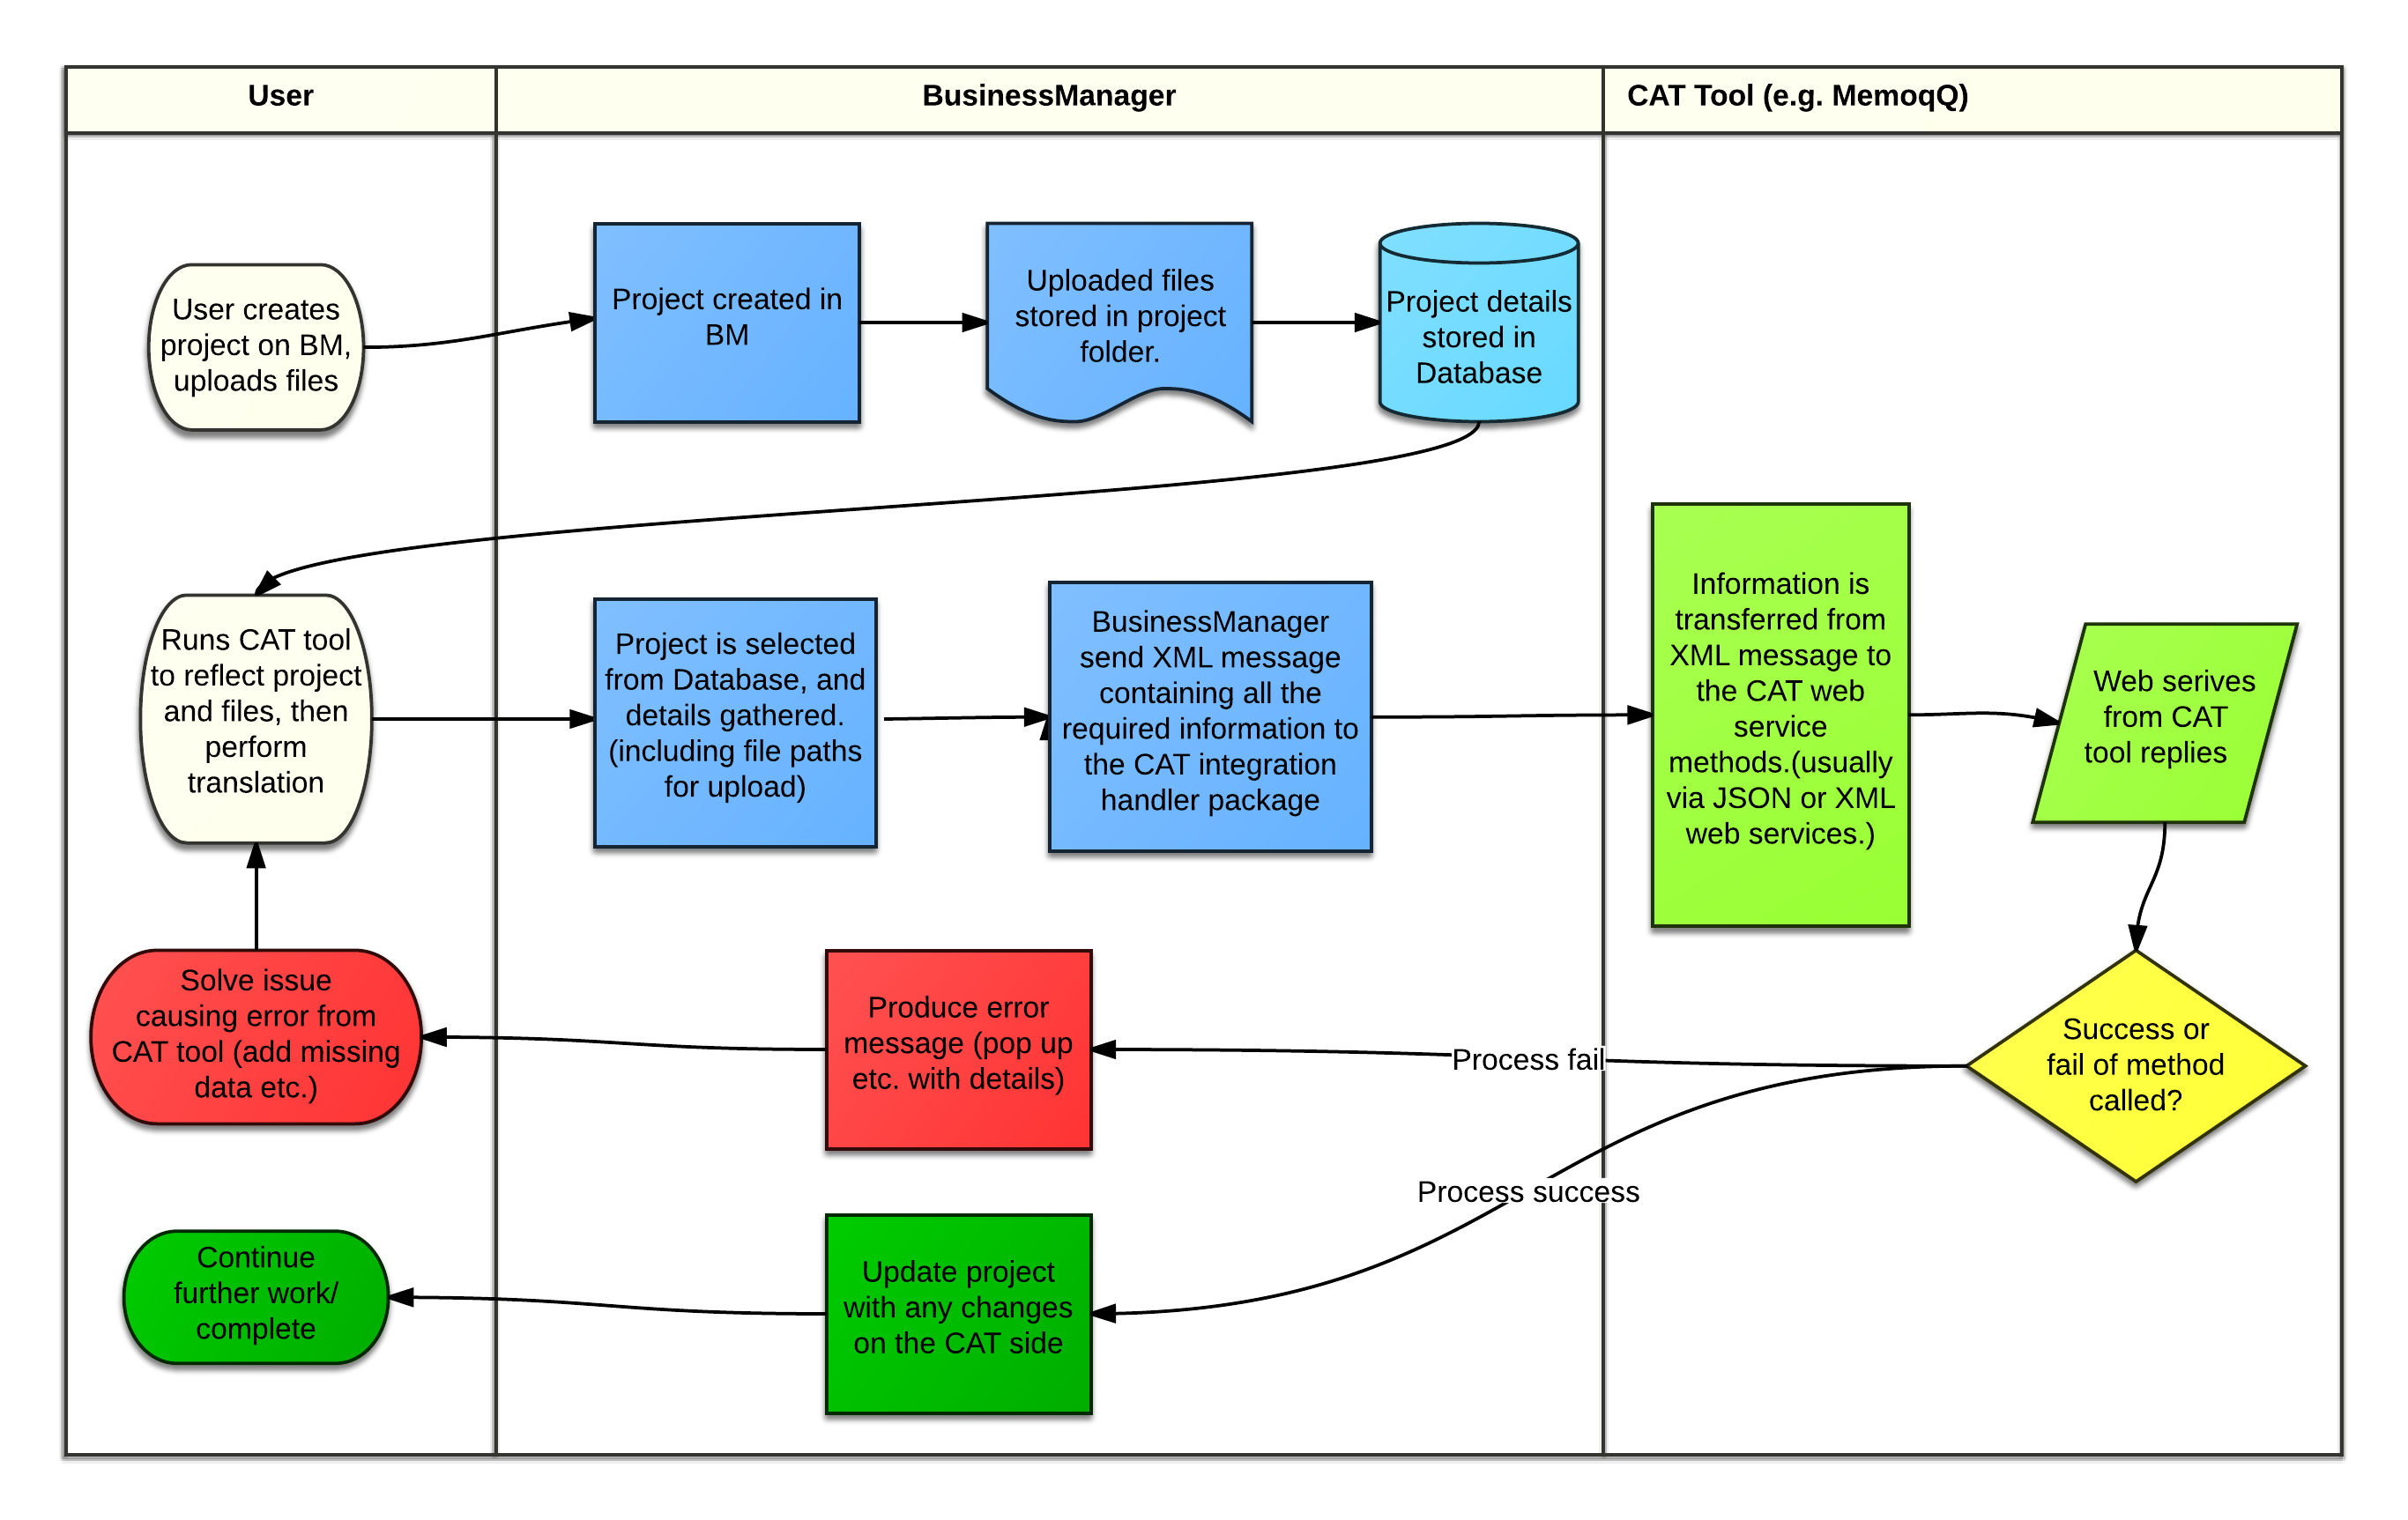
\includegraphics[scale=0.24]{cat}
    \caption{General means of CAT connectivity with BusinessManager.}
     \label{fig:cat}
\end{figure}
\end{landscape}

\begin{landscape}
\begin{figure}[p]
    \centering
    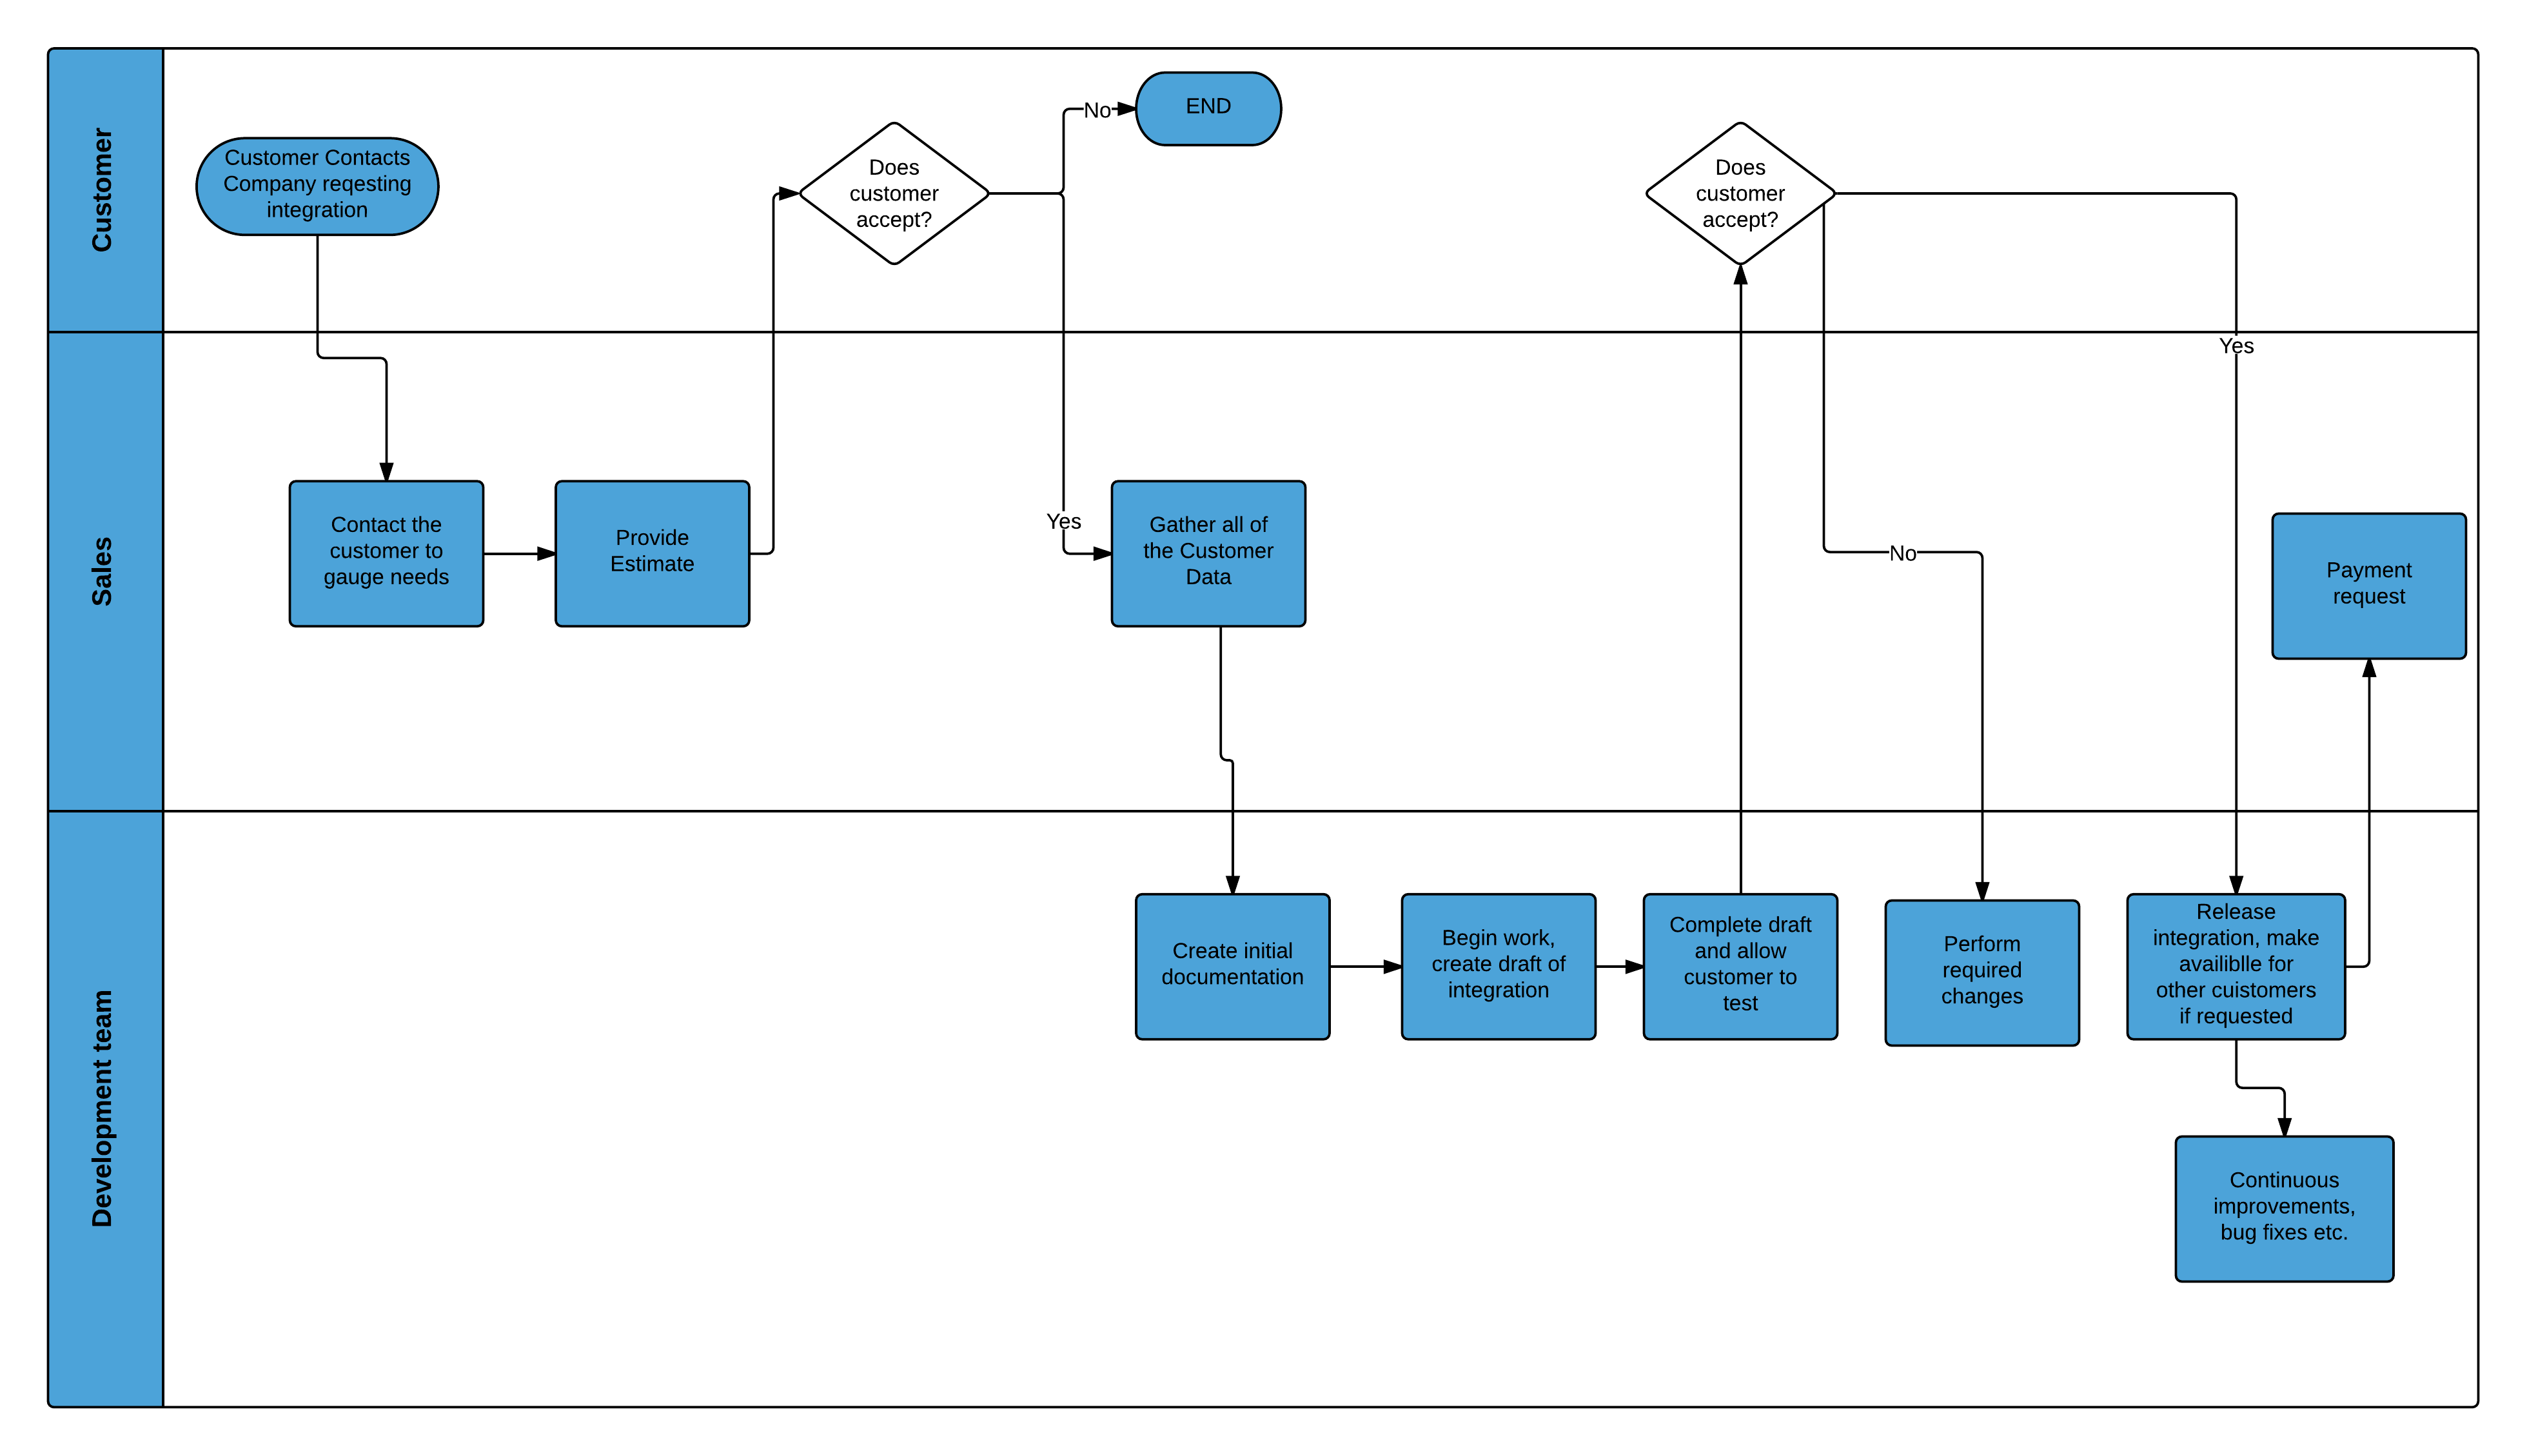
\includegraphics[scale=0.16]{sales}
    \caption{New CAT integration routine of work.}
     \label{fig:sales}
\end{figure}
\end{landscape}
%------------------------------------------------

%----------------------------------------------------------------------------------------
%   Critical Evaluation
%----------------------------------------------------------------------------------------

\section{Critical Evaluation}
In this section I have outlined a general evaluation of my performance, confidence and teamwork skills throughout the
time in my placement. Starting with the coding side of my work, when I first began my placement I didn’t think I was so
strong at Java, and especially envious about trying out the C\# language. During the beginning few months of my role, I
did find that although in the end the result performed the required task correctly, that it took longer than I wanted it
to, to implement. For instance, the use of Hash Maps and Hash Tables are quite abundant in the software, for storing
collections of objects such as users in the MySQL tables linked to BusinessManager. In these cases I had very little
experience and took quite some time to grasp. I found that I had to ask my head of department and colleagues quiet often
for help in the first couple of months.\\ \par \noindent
On the other half of this, once I had grasps the basics and understood why and where certain key programming paradigms
were used, the work itself became much easier to perform and also helped greatly in understanding how to implement new
features. To quickly summarise upon this, I believe my coding skills in Java have increased dramatically compared to
what they was before I went out on placement. As for C\# coding, because I had not done this before, it took a little
while longer to grasp, using more web tutorials at the beginning of my placement to get the basic fundamentals of the
language. Again, although I could always ask colleagues around me to help, I did feel more towards trying as much as
possible to learn more myself. By teaching some myself, this made me a better independent worker, and meant I did not
have to disturb or rely on colleagues as much.\\ \par \noindent
The other languages I used, JavaScript, MySQL, HTML and CSS were already very familiar to me, so looking at this from a
critical point of view I believe I handled well. I also think that in some cases what I learnt and used at the company
helped others there in the sense of any new found means coding methods.\\ \par \noindent
A very major point I should mention here is the style of the actual code, documentation and means of contact. Because
the company was based in Germany, most of the text involved in any of these was presented in the German language. At the
beginning of my placement I found this to be very difficult, and unusual. Because Java is based in English for all the
reserved words, it meant when reading lines of code or methods to find bugs, I first had to try and translate some
variable names before I could understand what they meant. Similarly, documentation and emails between staff the language
was almost always based in German which also made it quite hard for a native English speaker such as myself. As the year
progressed though, I did learn a great deal of the language from remembering phrases I had already translated. In the
first 3 months at Plunet, I also received some German lessons at a language school paid for by the company which helped
tremendously.\\ \par \noindent
Because of my lack of German In the beginning, I did code in English terms for variable names which did at points cause
confusion for some of my colleagues (they termed this ‘Genglish’). To keep consistency, I ensured later on to always
keep names in German and to try communicate more through German.\\ \par \noindent
This brings me to my final point in my critical evaluation, communication and teamwork skills. Again, being a German
company with almost all employees being German, this was the chosen language for all forms of communication internally.
In the very first few weeks, and after arriving in Germany knowing absolutely no German, I struggled to understand and
respond when in meetings and emails. This goes with the Skype messaging too, where most of the time I would use Google
Translate to help me understand communication though text sent to me. As time went on through my placement, and because
my head of department along with most other staff in the office speak good English, this was able to help me get to
grips with key words in German. This meant from around 5 months into my placement, I was confident enough to speak
German in the sprint meetings, and also within any emails or skype.

%------------------------------------------------

%----------------------------------------------------------------------------------------
%   Out of Work Life
%----------------------------------------------------------------------------------------

\section{Out-of-Hours Life}
As a short additional part of this report, the social life and out-of work activities should also be mentioned. Being in
another country meant I did not really know anyone out of work, so in order to make friends and also to make the most of
my time there, I joined a local badminton club. This meant a social every week, and regular playing sessions. This was
great for meeting people my own age, and meant I could also learn a little of the language there.\\ \par \noindent
When it came to socialising with work colleagues, there was quite regular events based around Würzburg, such as the Bier
Keller event, and Christmas markets. Going with work colleagues allowed me to enhance friendships between myself and
others. As a result of going to out of hour events and socialising made my knowledge of the German language generally
better.
\clearpage

%------------------------------------------------

%----------------------------------------------------------------------------------------
%	CONCLUSION
%----------------------------------------------------------------------------------------

\section{Conclusion}
For the final section in this report, my conclusions of the placement are outlined. Looking back at the general good and bad points of the whole
process of an industrial year, I can see what I would have done differently if I did it again. Firstly, knowing what I know now about seeking and
getting a placement, I have learnt that being more calm and patient can help a great deal when searching. For myself, after a few failed attempts at
applying for placements and feeling more doubtful each time, I know this should not affect the applicant. Instead, by continuing to apply for as many
opportunities as possible, yet making sure quality of application is still to a high standard, makes sure the best possible chance of getting a
placement.\\ \par \noindent
When it came to starting a placement, I found that although I had some good knowledge of the primary programming language that the application was
written in, it did not mean that I would understand and be able to begin my work straight away. This was because of many aspects; the programming
style, the algorithms used and even some of the language basics that I thought I knew but didn’t to the standards required at the time. I can also
conclude here that going on a placement in my field of study has gained me a great deal of valuable experience in programming not only specific to the
JavaEE format, but also as a whole. The style of coding and work process done at Plunet will surely continue to be used through my later pieces of
work in and out of university.\\ \par \noindent
I can also look at how moving to and working in another country has affected me. It has definitely opened my eyes to how other countries have both
major differences and also great similarities between how they do things. For me, Germany seemed a much organised place to be which fit in perfectly
with myself and my work. Being abroad also allowed me to learn a complete other language which I consider a bonus in the case of a placement.
Finally, if I were to offer advice to any other student thinking about or applying for placements, I would definitely recommend it, especially in
another country. Not only can I use the knowledge gained in the rest of the duration of my course, but also as part of my future career. This year has
also placed me in a good stead for applying for roles when completing my course.

%------------------------------------------------

\section{Document History}

\begin{tabular}{|l | l | p{3.2in} | l |}

\hline

Version & Date & Changes made to Document & Changed by \\

\hline

1.0 & 25/06/14 & Creation of first draft of document. & crh13\\

\hline

1.01 & 28/06/14 & Spelling error checking. & crh13\\

\hline

1.1 & 28/08/14 & Diagram amendments and 'out of hours' section added. & crh13\\

\hline

1.2 & 03/09/14 & Addition of references and proofread of document & crh13\\

\hline

2.0 & 08/09/14 & Release version & crh13\\

\hline

\end{tabular}

\vspace{6cm}

\begin{center}
\emph{Word count: 5446}
\end{center}

%------------------------------------------------

%----------------------------------------------------------------------------------------

\end{document}

%----------------------------------------------------------------------------------------